\section{Projektmanagement}
\label{sec:projektmanagement}

Im Folgenden wird die Projektgruppe vorgestellt und die Zusammenarbeit im Team sowie die dabei entstandenen Herausforderungen und Schwierigkeiten erläutert. Auf die Auswirkungen der Teamarbeit auf den Entwicklungsprozess wird im Anschluss eingegangen. Es wird der geplante, sowie der letztlich umgesetzte Entwicklungsprozess mit Aufgabenverteilung und Zeitplan vorgestellt.

%%%%%%%%%%%%%%%%%%%%%%%%%%%%%%%%%%%%%%%%%%%%%%%%%%%%%%%%%%%%%%%%%%%%%%%%%%%%%%%
%%%%%%%%%%%%%%%%%%%%%%%%%%%%%%%%%%%%%%%%%%%%%%%%%%%%%%%%%%%%%%%%%%%%%%%%%%%%%%%
%%%%%%%%%%%%%%%%%%%%%%%%%%%%%%%%%%%%%%%%%%%%%%%%%%%%%%%%%%%%%%%%%%%%%%%%%%%%%%%
% TEAMMITGLIEDER %%%%%%%%%%%%%%%%%%%%%%%%%%%%%%%%%%%%%%%%%%%%%%%%%%%%%%%%%%%%%%
%%%%%%%%%%%%%%%%%%%%%%%%%%%%%%%%%%%%%%%%%%%%%%%%%%%%%%%%%%%%%%%%%%%%%%%%%%%%%%%
\subsection{Projektgruppe und Teamarbeit}
\label{subsec:teammitglieder}

Das Softwareprojekt wurde mit vier Teammitgliedern begonnen. Dazu gehörten Alexa, Friedrich, Henry und Michael. Kurz vor Abschluss des Semesters hat Michael die Gruppe verlassen.

Die Tatsache, dass wir uns alle nicht kannten, weder aus vorangegangenen Kursen noch privat, stellte eine große Herausforderung in der Teamarbeit dar. Die Einschätzung der Zuverlässigkeit und des Engagements, sowie der Programmierkenntnisse war dadurch schwierig. Wir hatten alle unterschiedliche Vorerfahrungen und bevorzugten unterschiedliche Programmiersprachen. Diese Punkte erschwerten zu Beginn des Projekts die Einarbeitung und die Aufgabenverteilung.

Da wir nur vier Leute im Team waren, haben wir uns dazu entschieden keinen Projektleiter zu bestimmen, jeder sollte gleichermaßen Verantwortung für das Projekt übernehmen.


%%%%%%%%%%%%%%%%%%%%%%%%%%%%%%%%%%%%%%%%%%%%%%%%%%%%%%%%%%%%%%%%%%%%%%%%%%%%%%%
%%%%%%%%%%%%%%%%%%%%%%%%%%%%%%%%%%%%%%%%%%%%%%%%%%%%%%%%%%%%%%%%%%%%%%%%%%%%%%%
%%%%%%%%%%%%%%%%%%%%%%%%%%%%%%%%%%%%%%%%%%%%%%%%%%%%%%%%%%%%%%%%%%%%%%%%%%%%%%%
% TEAMMITGLIEDER %%%%%%%%%%%%%%%%%%%%%%%%%%%%%%%%%%%%%%%%%%%%%%%%%%%%%%%%%%%%%%
%%%%%%%%%%%%%%%%%%%%%%%%%%%%%%%%%%%%%%%%%%%%%%%%%%%%%%%%%%%%%%%%%%%%%%%%%%%%%%%
\subsection{Entwicklungsprozess}
\label{subsec:prozess}

Wir haben uns für das Hosting des Projekts bei Spline\footnote{\url{https://dev.spline.de/trac/CommonUnfold/browser/trunk}} entschieden. Zur Codeversionierung wird dabei SVN verwendet. Zusätzlich verwenden wir einen Bug-Tracker\footnote{\url{https://dev.spline.de/trac/CommonUnfold/}}, welcher direkt von Spline zur Verfügung gestellt wurde.\\

Als Programmiersprache haben wir uns auf \emph{Python} geeinigt, da der vorgegebene Prototyp in Python implementiert war. Nur einer aus unserer Projektgruppe, Henry, war sehr sicher in Python, alle anderen mussten sich erst einmal in die neue Programmiersprache einarbeiten. Bevor wir mit der Implementierung anfingen, hatte jeder zwei Wochen Zeit sich in die neue Programmiersprache einzuarbeiten. Für die Programmierung der grafischen Oberfläche haben wir \emph{TkInter} verwendet, ein Wrapper des Tk-Toolkits für Python.\\

Wir haben uns für kein festes Vorgehensmodell zur Softwareentwicklung, wie beispielsweise das Wasserfallmodell, SCRUM oder TDD, entschieden. Um die Kommunikation im Team und unseren Prozess zu unterstützen, sowie um eine regelmäßige Arbeitsweise aller zu forcieren, haben wir uns für die folgenden Prozesselemente und Regeln entschieden:

  \begin{description}
    \item[Lauffähige Version im Repository] Um ein effektives Arbeiten zu ermöglichen, sollten nur lauffähige Versionen ins SVN committed werden.
    \item[Wöchentliche Treffen] Bei regelmäßigen, wöchentlichen Treffen (meist freitags 14:00 Uhr) haben wir über den aktuellen Stand und über neue Aufgaben gesprochen. Hier wurden Tickets eingetragen und Aufgaben direkt verteilt und zugewiesen.
    \item[Trac und Tickets] Die neuen Aufgaben, welche gemeinsam formuliert und besprochen wurden, wurden im Trac als Ticket gemeinschaftlich eingetragen. Das Trac-System war zentraler Bestandteil unserer Zusammenarbeit und wurde im Verlaufe des gesamten Projekts kontinuierlich verwendet.
    \item[Definierte Aufgaben pro Person] Jeder konnte sich Aufgaben aus den Tickets auswählen und sich verbindlich zuweisen. Jeder hatte dann für gewöhnlich ein oder zwei Aufgaben \bzw Tickets bis zum nächsten Treffen zu erledigen.
    \item[Aussagekräftige Commits] Aussagekräftige \emph{Commit Messages} sollten das spätere Dokumentieren vereinfachen.
    \item[Bugs] Während der Implementierung gefundene Fehler sollten sofort im Trac eingetragen werden. 
  \end{description}

Das Softwareprojekt wurde innerhalb von 14 Wochen durchgeführt, vom 18. April 2011 bis 19. Juli 2011. Einen konkreten Zeitplan haben wir nicht erstellt. Jede Woche wurden Aufgaben definiert, welche bis zur darauf folgenden Woche \bzw bis zum nächsten Treffen erledigt werden sollten.\\

In Abbildung~\ref{fig:activePP} ist die Aktivität jedes Teilnehmers ersichtlich, gemessen an den Änderungen im SVN bestehend aus Changeset, erstellten und geschlossenen Tickets. In Abbildung~\ref{fig:activeTime} wird der zeitliche Verlauf und die Aktivität des Softwareprojekts deutlich.

\begin{figure}[htbp]
\centering
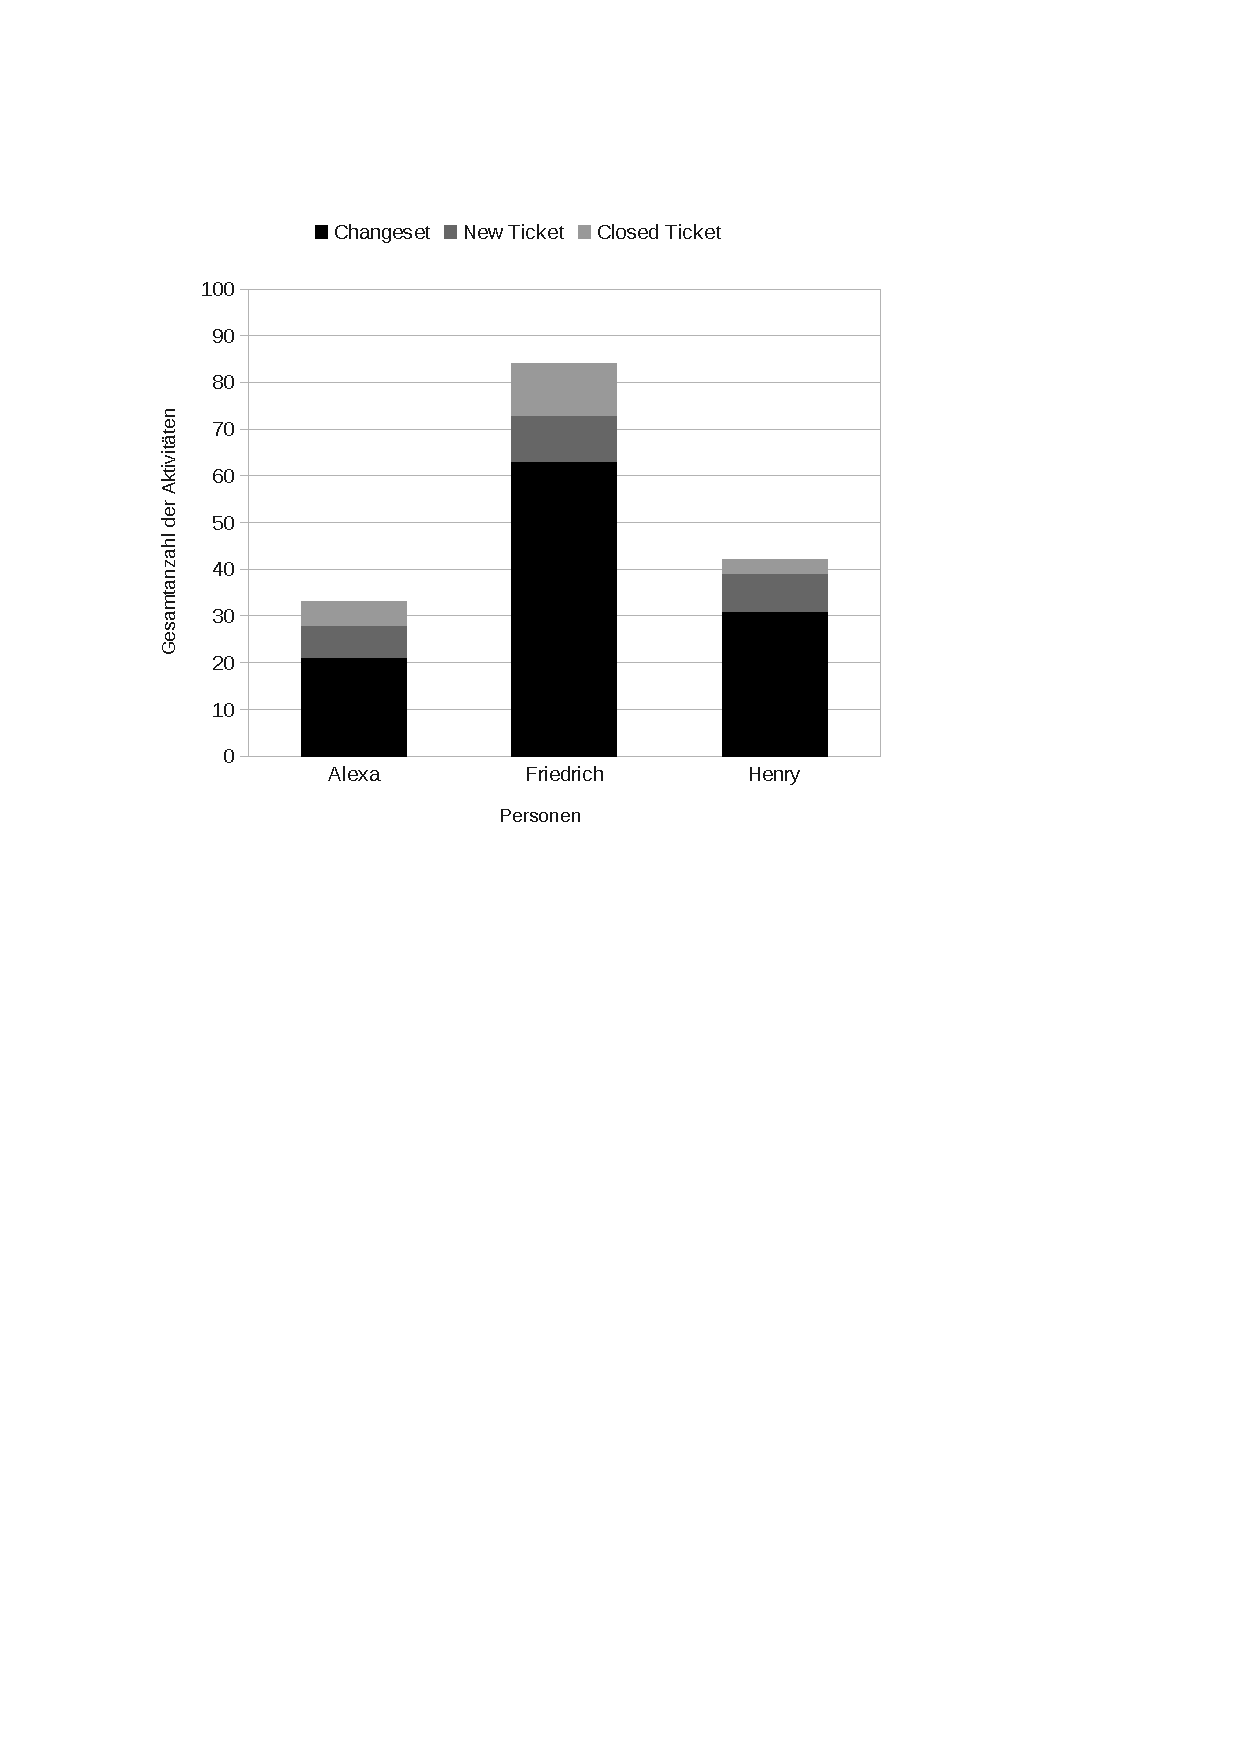
\includegraphics{03_pics/stat1.pdf}
\caption{Aktivität pro Person}
\label{fig:activePP}
\end{figure}

\begin{figure}[htbp]
\centering
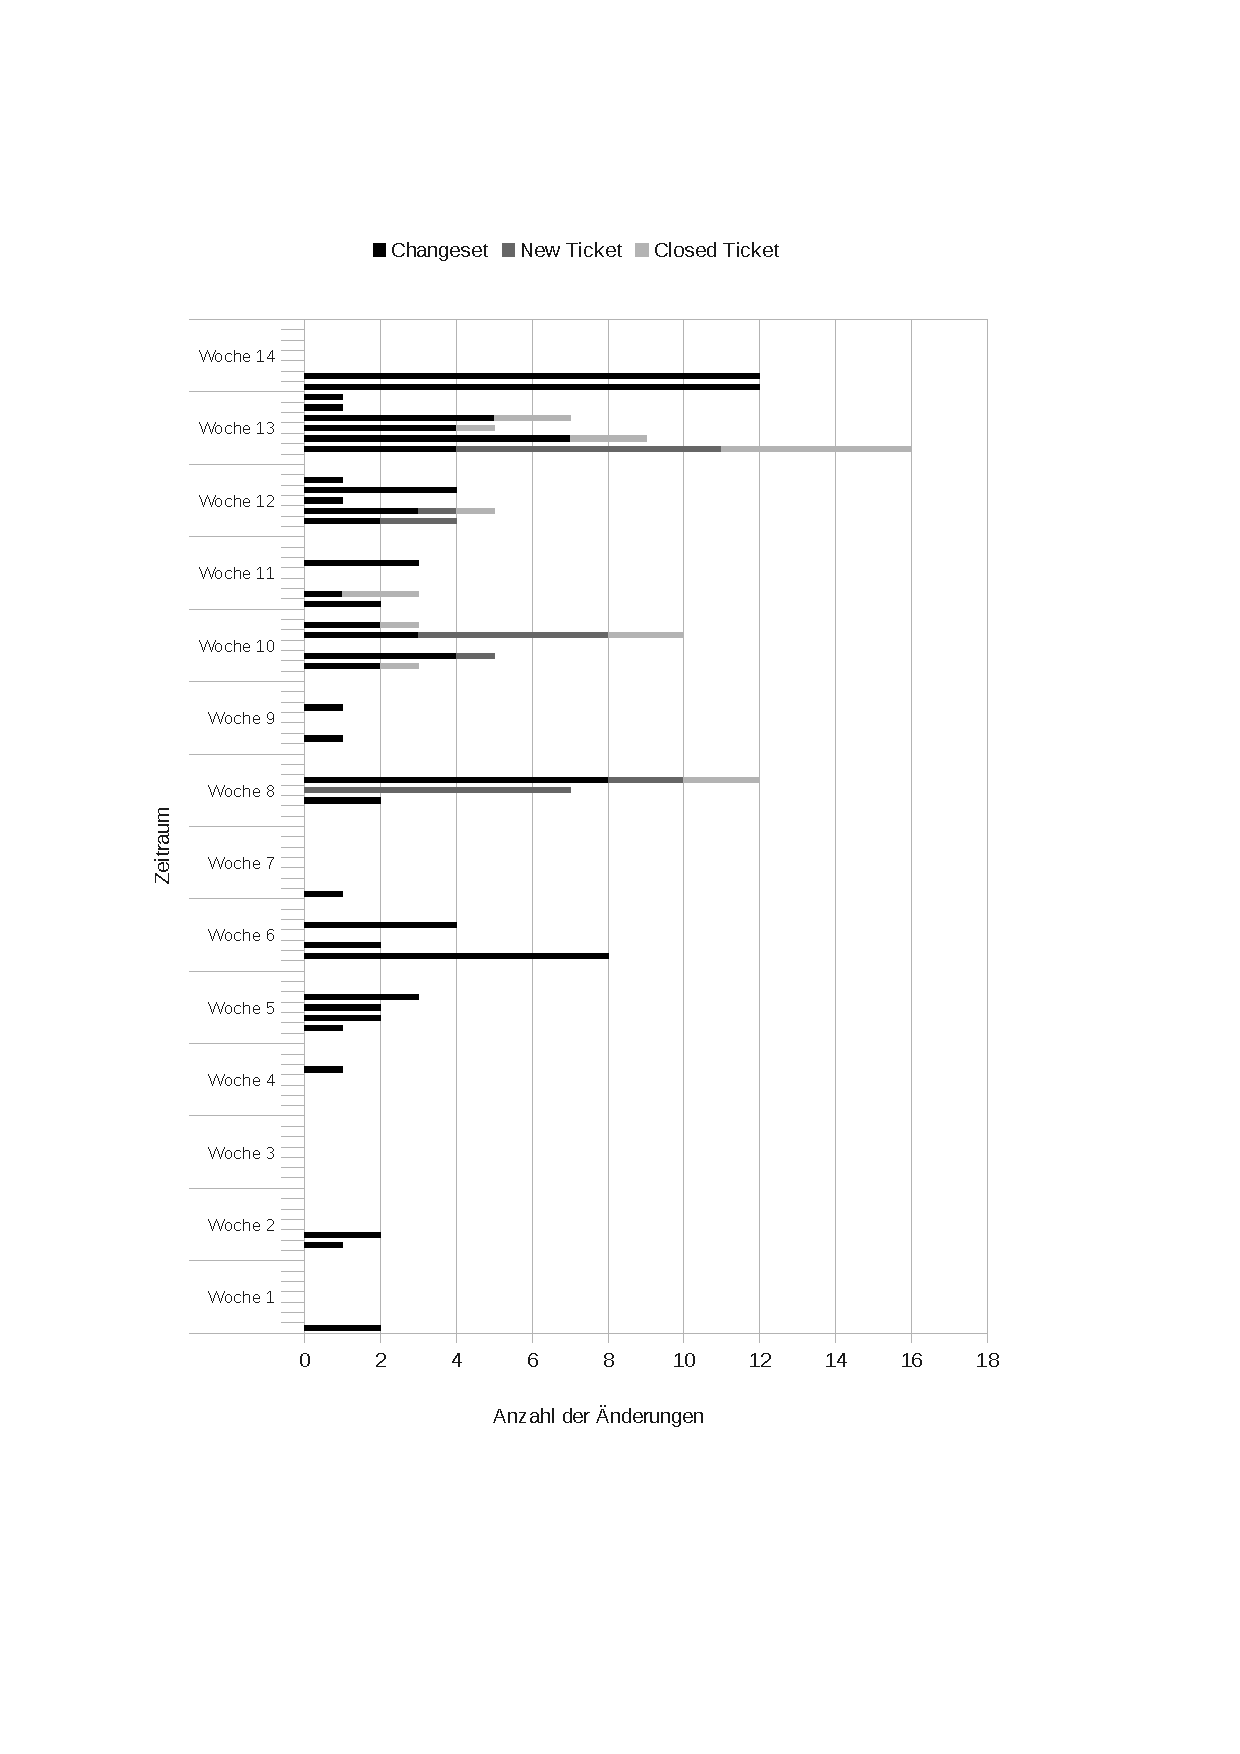
\includegraphics{03_pics/stat2.pdf}
\caption{Timeline}
\label{fig:activeTime}
\end{figure}


%%%%%%%%%%%%%%%%%%%%%%%%%%%%%%%%%%%%%%%%%%%%%%%%%%%%%%%%%%%%%%%%%%%%%%%%%%%%%%%
%%%%%%%%%%%%%%%%%%%%%%%%%%%%%%%%%%%%%%%%%%%%%%%%%%%%%%%%%%%%%%%%%%%%%%%%%%%%%%%
%%%%%%%%%%%%%%%%%%%%%%%%%%%%%%%%%%%%%%%%%%%%%%%%%%%%%%%%%%%%%%%%%%%%%%%%%%%%%%%
% FAZIT %%%%%%%%%%%%%%%%%%%%%%%%%%%%%%%%%%%%%%%%%%%%%%%%%%%%%%%%%%%%%%%%%%%%%%%
%%%%%%%%%%%%%%%%%%%%%%%%%%%%%%%%%%%%%%%%%%%%%%%%%%%%%%%%%%%%%%%%%%%%%%%%%%%%%%%
\subsection{Fazit zum Projektmanagement}
\label{subsec:fazitPM}

Für unser Softwareprojekt war unser Vorgehen als Gruppe nicht sehr optimal, hat aber trotzdem am Ende zu einem guten und lauffähigen Programm geführt. Trotzdem würden wir als Gruppe in einem neuen Projekt viele Dinge anders gestalten.

Ein erster Punkt wäre die Auswahl der Programmiersprache, wobei wir beim nächsten Mal eine Sprache wählen wollen, welche alle Teammitglieder ausreichend gut beherrschen, beispielsweise \emph{Java}. Diese Entscheidung würde unser radikales Vorgehen etwas entradikalisieren. Das Erstellen eines Zeitplans mit Meilensteinen und Arbeitspaketen ist ein Muss für das nächste Projekt.
Das Einsetzen eines Teamleiters, welcher nach außen hin die Kommunikation mit dem Professor und anderen Teams übernimmt und sich um die Organisation von Teamtreffen kümmert ist erstrebenswert. Um die Arbeitsmoral stets angenehm und positiv zu halten würden wir \emph{Coding Sessions} einplanen, wo sich alle Teammitglieder an einem Ort zum Programmieren treffen. Regelmäßige Protokolle sollten abwesenden Mitgliedern helfen auf dem aktuellen Stand der Entwicklung zu bleiben und Designentscheidungen nachzuvollziehen.
Wir haben darüber nachgedacht ein konkretes Vorgehensmodell zur Softwareentwicklung einzusetzen, beispielsweise \emph{Scrum}.